
\chapter{Introduction}
\label{chap:intro}

The widespread use of smart phones has led to the proliferation of a diverse range of location based services (LBSs). An important class of LBSs are spatial alarms that are triggered by the location of a moving user. Spatial alarm and variants in the Euclidean space and road networks have been recently addressed in the literature \cite{bamba},\cite{mur},\cite{roadalarm}. However, the moving path of a pedestrian is restricted by obstacles like buildings, fence and vehicles on road. In this thesis, we introduce personalized spatial alarms in the obstructed space. A pedestrian may plan to buy a medicine from a pharmacy while walking through a city or a tourist may want to have dinner at a restaurant while taking a scenic walk at an unfamiliar place. Spatial alarms enable users to know a point of interest (POI) such as a pharmacy or a restaurant comes within a specific range of the pedestrian. It is a personalized location based service as it can vary from user to user in terms of POI type and range. In this thesis we introduce an efficient approach to evaluate personalized spatial alarms efficiently in the obstructed space.

\vspace*{10pt}
A major challenge in processing spatial alarms in real time is it requires continuous evaluation with respect to the changed location of a moving user. Specifically, to trigger the spatial alarm for a pedestrian, an LBS needs to continuously check whether the specific type of POI is within the specific range of the current location of the pedestrian, which incurs high query processing overhead. Our approach to evaluate spatial alarm is simple and effective. We exploit geometric properties to refine the POI and obstacle search region in the total space and develop a technique to identify the area, i.e., reliable region, where a pedestrian's movement does not need to retrieve any new POI or obstacle from the LSP. Our approach keeps track of the area, i.e., known region, where POIs and obstacles are already retrieved and thereby avoids the retrieval of same POIs and obstacles from the LSPs databases. 
\vspace{10pt}

We aim to minimize device wake-ups and duplicate data transfer between client and server. Thus, we have formulated a safe region. As long as the user is within this region, no computation is needed to give the answer. Thus the safe region is a region in which the active alarms of a client remain unchanged. With the help of these three regions we provide an efficient approach to evaluate spatial alarms. It is noteworthy that spatial alarms are quite dissimilar to spatial range queries \cite{roadalarm}. Spatial alarms are based on a fixed location thus applying the techniques that are used in answering spatial range queries is both inefficient and wasteful for the two dominating reasons: Firstly, in a spatial range continuous re-evaluation of her location is needed in case of a mobile user. In contrast, spatial alarms need only be re-evaluated when the user is approaching a specific location. Secondly, in spatial range queries information about POIs in users vicinity is always important, whereas in spatial alarms, the information about POIs are relevant only if they are within certain range of the users. It is quite clear that applying spatial range query techniques in evaluating spatial alarms is going to result in wastage of resources. If we start to evaluate spatial alarms as soon as the user is on the move even if the user is far away from her desired location our efforts will be futile. 
\vspace*{10pt}



\section{Problem Setup}
Existing research has categorized spatial alarms into three types: Public, Shared and Private.\\
Public alarms are alarms which are active for every user within the system, such as an alarm must be sent to everyone within 100 meters of a building on fire. 
Private alarms are user defined alarms which can be viewed by the user, such as a user might set an alarm to alert her if she is within 100 meters of her favorite coffee shop.\\ 
Shared alarms are shared between specific groups of people. In the previous example if a user chooses to share the alarm for the coffee shop with some of her friends it becomes a shared spatial alarm.\\
In this thesis we are considering private alarms only. \\
In \cite{bamba}  spatial alarms has been categorized into three different types:
\begin{itemize}
 \item Moving subscriber with Static target
 \item Static subscriber with Moving target 
 \item Moving subscriber with Moving target 
\end{itemize}  
In this thesis we are only considering the first type, that is Moving subscriber with Static target.\\ 
In \cite{mur} spatial alarm region have been approximated by rectangular bounding box, in our approach we are considering the spatial alarm region as a circle with radius $r$.\\ \\
\textit{Obstructed Space Path Problem} \cite{deberg} denotes the problem of finding the shortest route between two query-points  in Obstructed Space where non-intersecting 2D polygons represent \textit{obstacles} and where the route does not traverse through any obstacles. The difference between obstructed distance and euclidean distance is clear from the figure \ref{fig:odist}. The length of the Obstructed route between points a and b is called the \textit{Obstructed Distance} between a and b, denoted by $dist_o(p_i,q)$.\\ \\

\begin{figure}[h]
  \includegraphics[width=\linewidth]{obstructed_distance.png}
  \caption{Obstructed Distance}
  \label{fig:odist}
\end{figure}
\vspace{2mm}


A \textbf{Spatial Alarm Query in Obstructed Space} is formally defined as follows:
%\begin{defn}
Given a moving query point q and a range r for an alarm, a Spatial Alarm Query returns $\forall p_i \in P=\left\lbrace p_1,p_2,p_3...p_n\right\rbrace  $ which have $dist_o(p_i,q)<r $
%\end{defn}
% The GETALLPOI(R,P) and GETOBSTACLESET(q,R,O) functions populates the sets P and O with the POIs and obstacles respectively within the distance R from the client's current location.
%\\MAKEVISGRAPH(P,O) returns the \textit{visibility graph} V$_G$ with the set of POIs P and Obstacles O.
%A \textbf{Visibility Graph} is a graph $V_G(V,E)$ where each v $\in$ V is either a POI or a Data point and for each (u,v)$ \in$ V, there is an edge e between u and v if and only if it does not interesect with any obstacles i.e. u and v are \textit{visible} to each other. \\
%EUCLIDEANDIST(q1,q2) returns the euclidean space distance between two points q1 and q2.\\
%CHECKNEWPOI(q,$r_k$,P) \\
%ALARMUSER(P$_i$) triggers an alarm to the user for the alarm $P_i$. \\  
% Single-column table

\section{Preliminaries}
Spatial alarms are location-based, user-defined triggers which will possibly shape the future mobile application computations. They are distinct from spatial range query and do not need immediate evaluation after the user has activated them. The spatial alarm evaluation strategies are judged based on two features, High accuracy and High system scalability. High accuracy refers to the quality that guaranties no alarms are missed. And High scalability is the feature that ensures that the system can adapt to a large number of spatial alarms.\\
In this thesis, We propose a novel approach to evaluate spatial alarms in obstructed space which ensures both High accuracy and High scalability.

We define three different type of regions: \textit{Known Region},\textit{Reliable Region} and \textit{Safe Region}\\ \\

\textbf{Known Region:} \\
                    \hspace*{4cm}The region within which all POIs (alarms) and  obstacles are known to the client.
We define two different known regions for the POIs and the obstacles. Both of the known regions are represented by a parabola whose focus point is the users location q,with the equation $y^2=4ax$ where $a=mr$ which is bounded by a straight line. \\ \\

\begin{figure}[h]
  \includegraphics[width=\linewidth]{Regions.png}
  \caption{Definition of Regions}
  \label{fig:defregion}
\end{figure}



\textbf{Reliable Region:}\\
\hspace*{4cm} Within which region, no further query to the server has to be done to compute a consistent set of answers, that is termed as a reliable region. The reliable region is also a parabolic region bounded by a straight line,where each bounding point of the parabolic curve is at a distance r from the known regions parabolic curve. $ \forall p_i=(x,y) $ in the known region, $ \forall p_j=(x_r,y_r) $ in the reliable region, $ dist_E(p_i,p_j)\geq r $ By this definition no further queries to the server has to be done to compute a consistent set of answers. Because, for any $q =p_j$ $ dist_E(q,p_j) \geq r$ where $p_j$ is a point on the boundary of the reliable region. And for all other points $ p_i $ inside the reliable region $  dist_E(q,p_i)>r$ \\ 


\textbf{Safe Region:}\\ 
\hspace*{3cm} A safe region is the region located inside reliable region within which the answer set of POIs remains unchanged for a moving client. We will denote the radius of the safe region as $r_{safe}$. Given the user's previous location $P_1$ and the current location $P_2$, if $(P_1 - P_2) < r_{safe}$, then no recalculation is needed to compute the answer. If the safe region surpasses the reliable region at some points. \\ 



\begin{table}[h]
\centering 

\caption{Symbol Table}
\begin{tabular}{|c|c|} \hline
Symbols&Meaning \\ \hline
P &  A set of POIs\\ \hline
O & A set of Obstacles\\ \hline
q & The location of user\\ \hline
$r$ & The alarming range\\ \hline
$V_{G}$       & A visibility Graph\\ \hline
$dist_E$(p,q) & The euclidean distance between points p and q\\ \hline
$dist_O$(p,q) & The obstructed distance between points p and q\\ \hline
$r_{safe}$    & The radius of safe region\\ \hline
$m$           & A real number in the range $[2,\infty)$ \\ \hline
$n$           & A real number in the range $[1,\infty) $  \\ \hline
$\theta_i $   & The angle between consecutive path segments \\ \hline 
$ S $         & The users path history as a set of straight lines \\ \hline
$(m_i,c_i,l_i)$ & A line with slope $m_i$, intercept $c_i$ and length $l_i$ \\ \hline

\end{tabular}
\end{table}
\vspace*{12pt}

The key idea of our approach is to calculate a dynamic \textit{safe region}, within which no computation has to be done to provide an accurate alarm trigger. We will use an R-tree structure to index both obstacles and POI's in our approach. Our spatial alarm processing system has two different modes for efficient and effective processing of spatial alarms,namely, Bandwidth saving mode and Computational Cost Saving mode.\\

We assume that the system is based on a client-server architecture and the POIs as well as the obstacles are stored using independent R-trees at the server. We also assume that all users have access to some sort of localization service such as GPS or Wi-Fi that queries the server with the client's pinpoint location. Here, the client application is a thin-weight application that communicates with the server on any specified event to retrieve necessary information about POIs and the obstacles. We assume that the user can use any device such as smart-phones or PDA.
%section starts

\section{Contributions}

 Our approach accounts for both accuracy and efficiency by focusing on (1) Not missing any alarms in user's proximity (2) Avoiding multiple retrival of duplicate data from the database (3) Minimizing communication between the LSP and client. In summary the our main contributions are: 
\begin{itemize}
\setlength\itemsep{0em}
\item We introduce spatial alarm queries in the obstructed space for mobile users.
\item We exploit geometric properties to refine the POI and obstacle search region in the total space and develop a technique for the client device to identify the area where a pedestrians moevment does not need to retrive any POI or obstacle from the LSP.
\item We provide an algorithm to calculate a dynamically changing region to accurately evaluate spatial alarm queries without any computation.
\item We provide an extensive experimental analysis to compare the efficiency of our approach with other naive approaches based on different parameters.
\end{itemize}

\vspace*{10pt}


\section{Thesis Organization}
\label{sec:org}

\vspace*{5pt}

The next chapters are organized as follows. In Chapter \ref{chp:relworks}, related works are discussed. In Chapters \ref{chap:naivesoln} and \ref{chap:ourapp}, we present a naive approach and our approach, respectively, to evaluate spatial alarm queries in the obstructed space. Chapter~\ref{chp:exp} shows the experimental results for our proposed algorithm. Finally, in Chapter~\ref{chp:conclusion}, we conclude with future research directions.


